% REMEMBER TO SET LANGUAGE!
\documentclass[a4paper,10pt,english]{article}
\usepackage[utf8]{inputenc}
\usepackage[english]{babel}
% Standard stuff
\usepackage{amsmath,graphicx,varioref,verbatim,amsfonts,geometry}
% colors in text
\usepackage[usenames,dvipsnames,svgnames,table]{xcolor}
% Hyper refs
\usepackage[colorlinks]{hyperref}

% Document formatting
\setlength{\parindent}{0mm}
\setlength{\parskip}{1.5mm}

%Color scheme for listings
\usepackage{textcomp}
\definecolor{listinggray}{gray}{0.9}
\definecolor{lbcolor}{rgb}{0.9,0.9,0.9}

%Listings configuration
\usepackage{listings}
%Hvis du bruker noe annet enn python, endre det her for å få riktig highlighting.
\lstset{
	backgroundcolor=\color{lbcolor},
	tabsize=4,
	rulecolor=,
	language=python,
        basicstyle=\scriptsize,
        upquote=true,
        aboveskip={1.5\baselineskip},
        columns=fixed,
	numbers=left,
        showstringspaces=false,
        extendedchars=true,
        breaklines=true,
        prebreak = \raisebox{0ex}[0ex][0ex]{\ensuremath{\hookleftarrow}},
        frame=single,
        showtabs=false,
        showspaces=false,
        showstringspaces=false,
        identifierstyle=\ttfamily,
        keywordstyle=\color[rgb]{0,0,1},
        commentstyle=\color[rgb]{0.133,0.545,0.133},
        stringstyle=\color[rgb]{0.627,0.126,0.941}
        }
        
\newcounter{subproject}
\renewcommand{\thesubproject}{\alph{subproject}}
\newenvironment{subproj}{
\begin{description}
\item[\refstepcounter{subproject}(\thesubproject)]
}{\end{description}}

%Lettering instead of numbering in different layers
%\renewcommand{\labelenumi}{\alph{enumi}}
%\renewcommand{\thesubsection}{\alph{subsection}}

%opening
\title{AST1100 - Week 1}
\author{Gunnar Lange}
\begin{document}
\maketitle
\section*{Exercise 1}
\subsection*{A.1}
Using a simple python script:\\
\lstinputlisting{1A1.py}
\textbf{1)} 0.3085\\
\linebreak
\textbf{2)} Symmetrical around $\sigma$ so 0.68\\
\linebreak
\textbf{3)} $(0.3085)^7=2.659\times 10^{-4}$\\
\linebreak
\textbf{4)} Binomial experiment so:
$$P(4, 7, 0,.5)={7\choose 4}(0.3085)^4(1-0.3085)^3=0.105$$
\pagebreak
\subsection*{A.2}
\subsubsection*{1)}
Again, a simple Python Script solves 1a)-1e):
\lstinputlisting{1A21.py}
This creates this figure:\\
\begin{figure}[h!]
        \centering 
        %Scale angir størrelsen på bildet. Bildefilen må ligge i samme mappe som tex-filen. 
        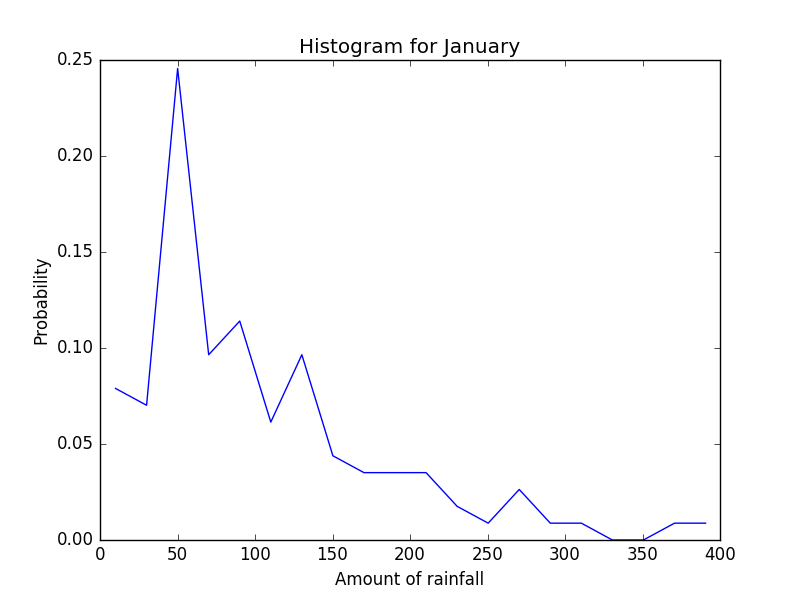
\includegraphics[scale=0.5]{january.png} 
        \caption{Histogram for January}
        %Label gjør det enkelt å referere til ulike bilder.
        \label{fig:January}
\end{figure}
\textbf{f)} The rainfall distribution is fairly clearly non-Gaussian.\\
\pagebreak
\textbf{g)} Trying February gives the following figure which again is clearly non-Gaussian.
\begin{figure}[h!]
        \centering 
        %Scale angir størrelsen på bildet. Bildefilen må ligge i samme mappe som tex-filen. 
        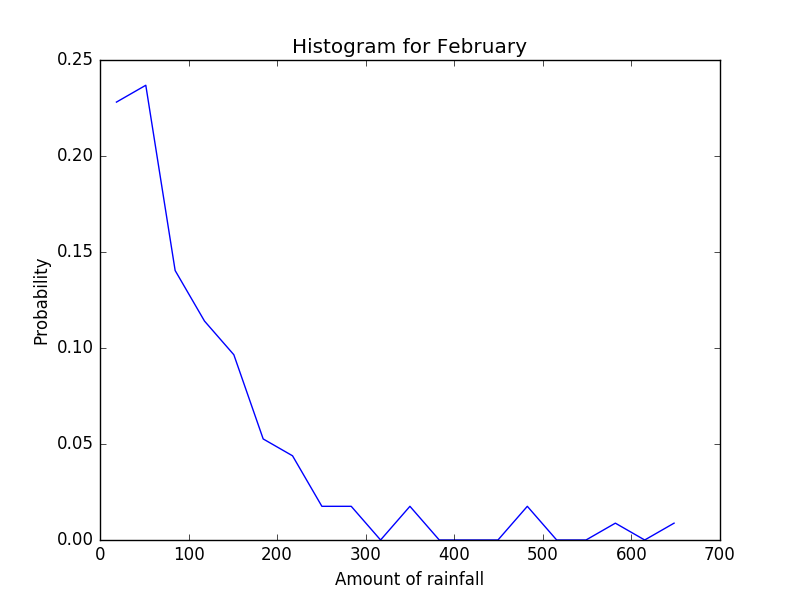
\includegraphics[scale=0.5]{February.png} 
        \caption{Histogram for February}
        %Label gjør det enkelt å referere til ulike bilder.
        \label{fig:February}
\end{figure}
\subsubsection*{2)}
Once again a straightforward Python script:
\lstinputlisting{1A22.py}
I.e. the probability is the probability of getting a specified bin.
\subsubsection*{3)}
Again a straightforward Python script:\\
\lstinputlisting{1A23.py}
\subsubsection*{4)}
Again a simply Python script gives:\\
\lstinputlisting{1A24.py}
With the following figure, which certainly looks more Gaussian:
\begin{figure}[h!]
        \centering 
        %Scale angir størrelsen på bildet. Bildefilen må ligge i samme mappe som tex-filen. 
        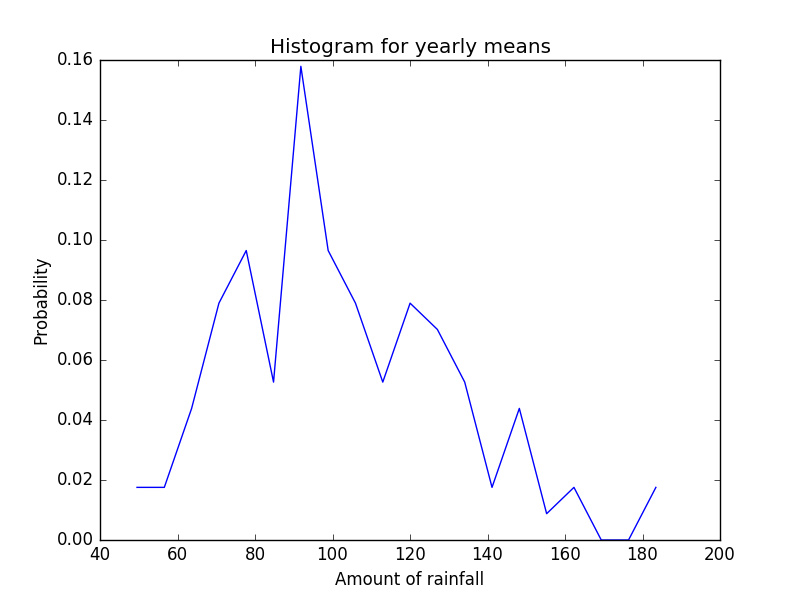
\includegraphics[scale=0.5]{yearly_means.png} 
        \caption{Histogram for February}
        %Label gjør det enkelt å referere til ulike bilder.
        \label{fig:Yearly_Means}
\end{figure}
\subsubsection*{5)}
A Python script:
\lstinputlisting{1A24.py}
Producing the following plot:
\begin{figure}[h!]
        \centering 
        %Scale angir størrelsen på bildet. Bildefilen må ligge i samme mappe som tex-filen. 
        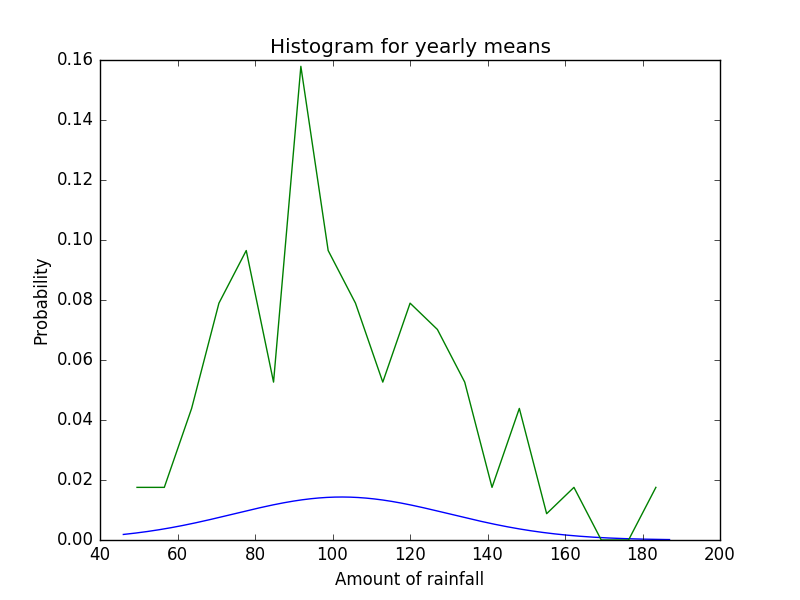
\includegraphics[scale=0.5]{yearly_means_Gauss.png} 
        \caption{Histogram for yearly means}
        %Label gjør det enkelt å referere til ulike bilder.
        \label{fig:Yearly_Means}
\end{figure}
Something is wrong. I do not have time to figure that out now.\\
\subsection*{A.3}
\subsubsection*{1)}
This is a direct application of the probability calculator, giving:
$$\sigma = 0.682 \quad 2\sigma=0.954, \quad 3\sigma = 0.997, \quad 4\sigma = 0.9998, \quad 5\sigma =0.9998$$
Presumable numerical errors were too large in the last one.
\subsubsection*{2)}
Definition of FWHM: width at $f(x)=\pm \mathrm{max}/2$. Recalling the definition of the Gaussian:
$$f(x)=\frac{1}{\sigma \sqrt{2\pi}}e^{-\frac{(x-\mu)^2}{2\sigma^2}}$$
The max is at $x=\mu$, where $f(x)=1/\sigma \sqrt{2\pi}$, so I must investigate where the Gaussian is half that value:
$$\frac{1}{2\sigma \sqrt{2\pi}}=\frac{1}{\sigma \sqrt{2\pi}}e^{-\frac{(x-\mu)^2}{2\sigma^2}}$$
$$\ln 2 = \frac{(x-\mu)^2}{2\sigma^2}$$
$$x=\mu \pm\sqrt{2\sigma^2 \ln 2}$$
To find the width, I must subtract the larger of these values from the smaller one:
$$x_2-x_1=FWHM=\mu+\sqrt{2\sigma^2 \ln 2}-(\mu - \sqrt{2\sigma^2 \ln 2})=2\sqrt{2\sigma^2 \ln 2}=\sigma  \sqrt{8\ln 2}$$
From which it follows that:
$$\sigma=\frac{FWHM}{\sqrt{8\ln 2}}$$
As was to be shown.
\subsection*{A.4}
\subsubsection*{1)}
A simple Python script, implementing the Maxwell-Boltzmann distribution, gives the answer quickly:
\lstinputlisting{1A41.py}
Which gives: $n(v)=5.51\times 10^{23}$.
\subsubsection*{2)}
This is of course exactly the same calculation, only substituting the function. I will not do this now.
\subsection*{A.5}
\subsubsection*{1)}
Starting from equation 6 as suggested:
$$\langle v \rangle = \int_0^{\infty} v\left(\frac{m}{2\pi k T}\right)^{3/2} e^{-\frac{mv^2}{2kT}}4\pi v^2 dv$$
I will now attempt to comptute this integral. A nautral way to begin is to make the substitution:
$$u=v^2, \quad \frac{du}{dv}=2v \implies dv = \frac{du}{2v}$$
Giving:
$$\langle v \rangle = \left(\frac{m}{2\pi k T}\right)^{3/2} \int_0^{\infty} 2\pi u e^{-\frac{mu}{2kT}}du$$
Now let:
$$\beta = \frac{m}{2kT}, \quad v=\beta u, \quad du=\frac{dv}{\beta}$$
Transforming the integral into:
$$\langle v \rangle = \left(\frac{m}{2\pi k T}\right)^{3/2}2\pi\int_0^\infty\frac{ve^{-v}}{\beta^2}dv=\frac{1}{\beta^2}\left(\frac{m}{2\pi k T}\right)^{3/2}=\sqrt{\frac{8kT}{m\pi}}$$ 
\subsubsection*{2)}
Starting from equation 11 as suggested:
$$P=\frac{n}{3}\int_0^{\infty}\frac{p^2}{m}\left(\frac{1}{2\pi mk T}\right)^{3/2}e^{-\frac{1}{2}\frac{p^2}{mkT}}4\pi p^2dp$$
I want to arrive at:
$$P=nkT$$
I begin by taking all constants outside:
$$P=\frac{4\pi n}{3m}\left(\frac{1}{2\pi mkT}\right)^{3/2}\int_0^{\infty} p^4 e^{-\frac{1}{2}\frac{p^2}{mkT}}dp$$
Let $u=p^2$. Then:
$$\frac{du}{dp}=2p, \quad dp=\frac{du}{2p}$$
Then the integral becomes:
$$\int_0^{\infty}\frac{u^{3/2}}{2}e^{-\frac{1}{2}\frac{u}{mkT}}du$$
Let:
$$\beta = \frac{1}{2mkT}, \quad v=\beta  u, \quad du=\frac{dv}{\beta}$$
Then the integral transforms to:
$$\int_0^{\infty} \frac{v^{3/2}}{2\beta^{5/2}}e^{-v}dv=\frac{3\sqrt{\pi}}{8\beta^{5/2}}$$
Giving, finally:
$$P=\frac{4\pi n}{3m}\left(\frac{1}{2\pi mkT}\right)^{3/2}\frac{3\sqrt{\pi}(2mkT)^ {5/2}}{8}$$
$$P=\frac{n}{2m}\left(2mkT\right)=nkT$$
As was to be shown.
\subsubsection*{3)}
I need to use the RMS of the speed squared. To find the average of the square of the speed, I thus need to compute:
$$\langle E_k \rangle=\langle \frac{1}{2}mv^2 \rangle = \int_0^{\infty} \frac{1}{2}mv^2P(v) dv=\int_0^{\infty}v^4\left(\frac{m}{2\pi k T}\right)^{3/2}e^{-\frac{mv^2}{2kT}}2m\pi dv$$
$$\langle E_k \rangle=\frac{2\pi m^{5/2}}{(2\pi k T)^{3/2}}\int_0^{\infty} v^4e^{-\frac{mv^2}{2kT}} dv$$
Using a standard strategy for the integral:
$$u=v^2, \quad \frac{du}{dv}=2v, \quad dv=\frac{du}{2v}$$ 
$$\int_0^{\infty}\frac{u^{3/2}}{2}e^{-\frac{mu}{2kT}}du$$
Let:
$$\beta=\frac{m}{2kT}, \quad x=\beta u, \quad du=\frac{dx}{\beta}$$
$$\int_0^{\infty}\frac{u^{3/2}}{2}e^{-\frac{mu}{2kT}}=\int_0^{\infty}\frac{x^{3/2}}{2\beta^{5/2}}e^x dx=\frac{3\sqrt{\pi}}{8\beta^{5/2}}$$
Putting this all together then:
$$\langle E_k \rangle = \frac{2\pi m^{5/2}}{(2\pi k T)^{3/2}}\frac{3\sqrt{\pi}}{8\beta^{5/2}}= \frac{2\pi m^{5/2}}{(2\pi k T)^{3/2}}\frac{3\sqrt{\pi}(2kT)^{5/2}}{8m^{5/2}}=\frac{3}{2}kT$$
As was to be shown.
\subsection*{A.6}
I do not have a home planet yet, so I will do this for the earth. Equating potential and kinetic energy gives:
$$\frac{1}{2}mv_{esc}=\frac{GmM}{R^2}$$
Giving:
$$v_{esc}=\sqrt{\frac{2GM}{R}}$$
\end{document}

